\documentclass[a4paper, top=10mm]{article}
%for writing from the top
\usepackage{fullpage}
%for math
\usepackage{amsmath}
\usepackage{mathrsfs}
\usepackage{amsthm}
%for images
\usepackage{graphicx}
%for color
\usepackage{xcolor}
%for title
\title{\textbf{\huge{New Santa's Sleigh}}}
\author{Enigma n\textsuperscript{o}7}
\date{14\textsuperscript{th} December 2023}

\newtheorem*{hint}{Hint}

\addtolength{\voffset}{-2cm}
\addtolength{\textheight}{5cm}


\begin{document}
	\maketitle
	
	Santa's magical reindeer are getting old.
	In order to have no disruption in the distribution of presents when the reindeer can no longer fly, Santa is testing a new model of sleigh from the future: a laser-powered sleigh.
	
	The concept is simple: Santa Clause needs to ask the elves to construct towers at regular intervals.
	They will take it in turns to propel the sleigh via ultra-powerful lasers.
	To prevent the sled from disintegrating, it is fitted with a shield at the rear.
	
	\begin{center}
		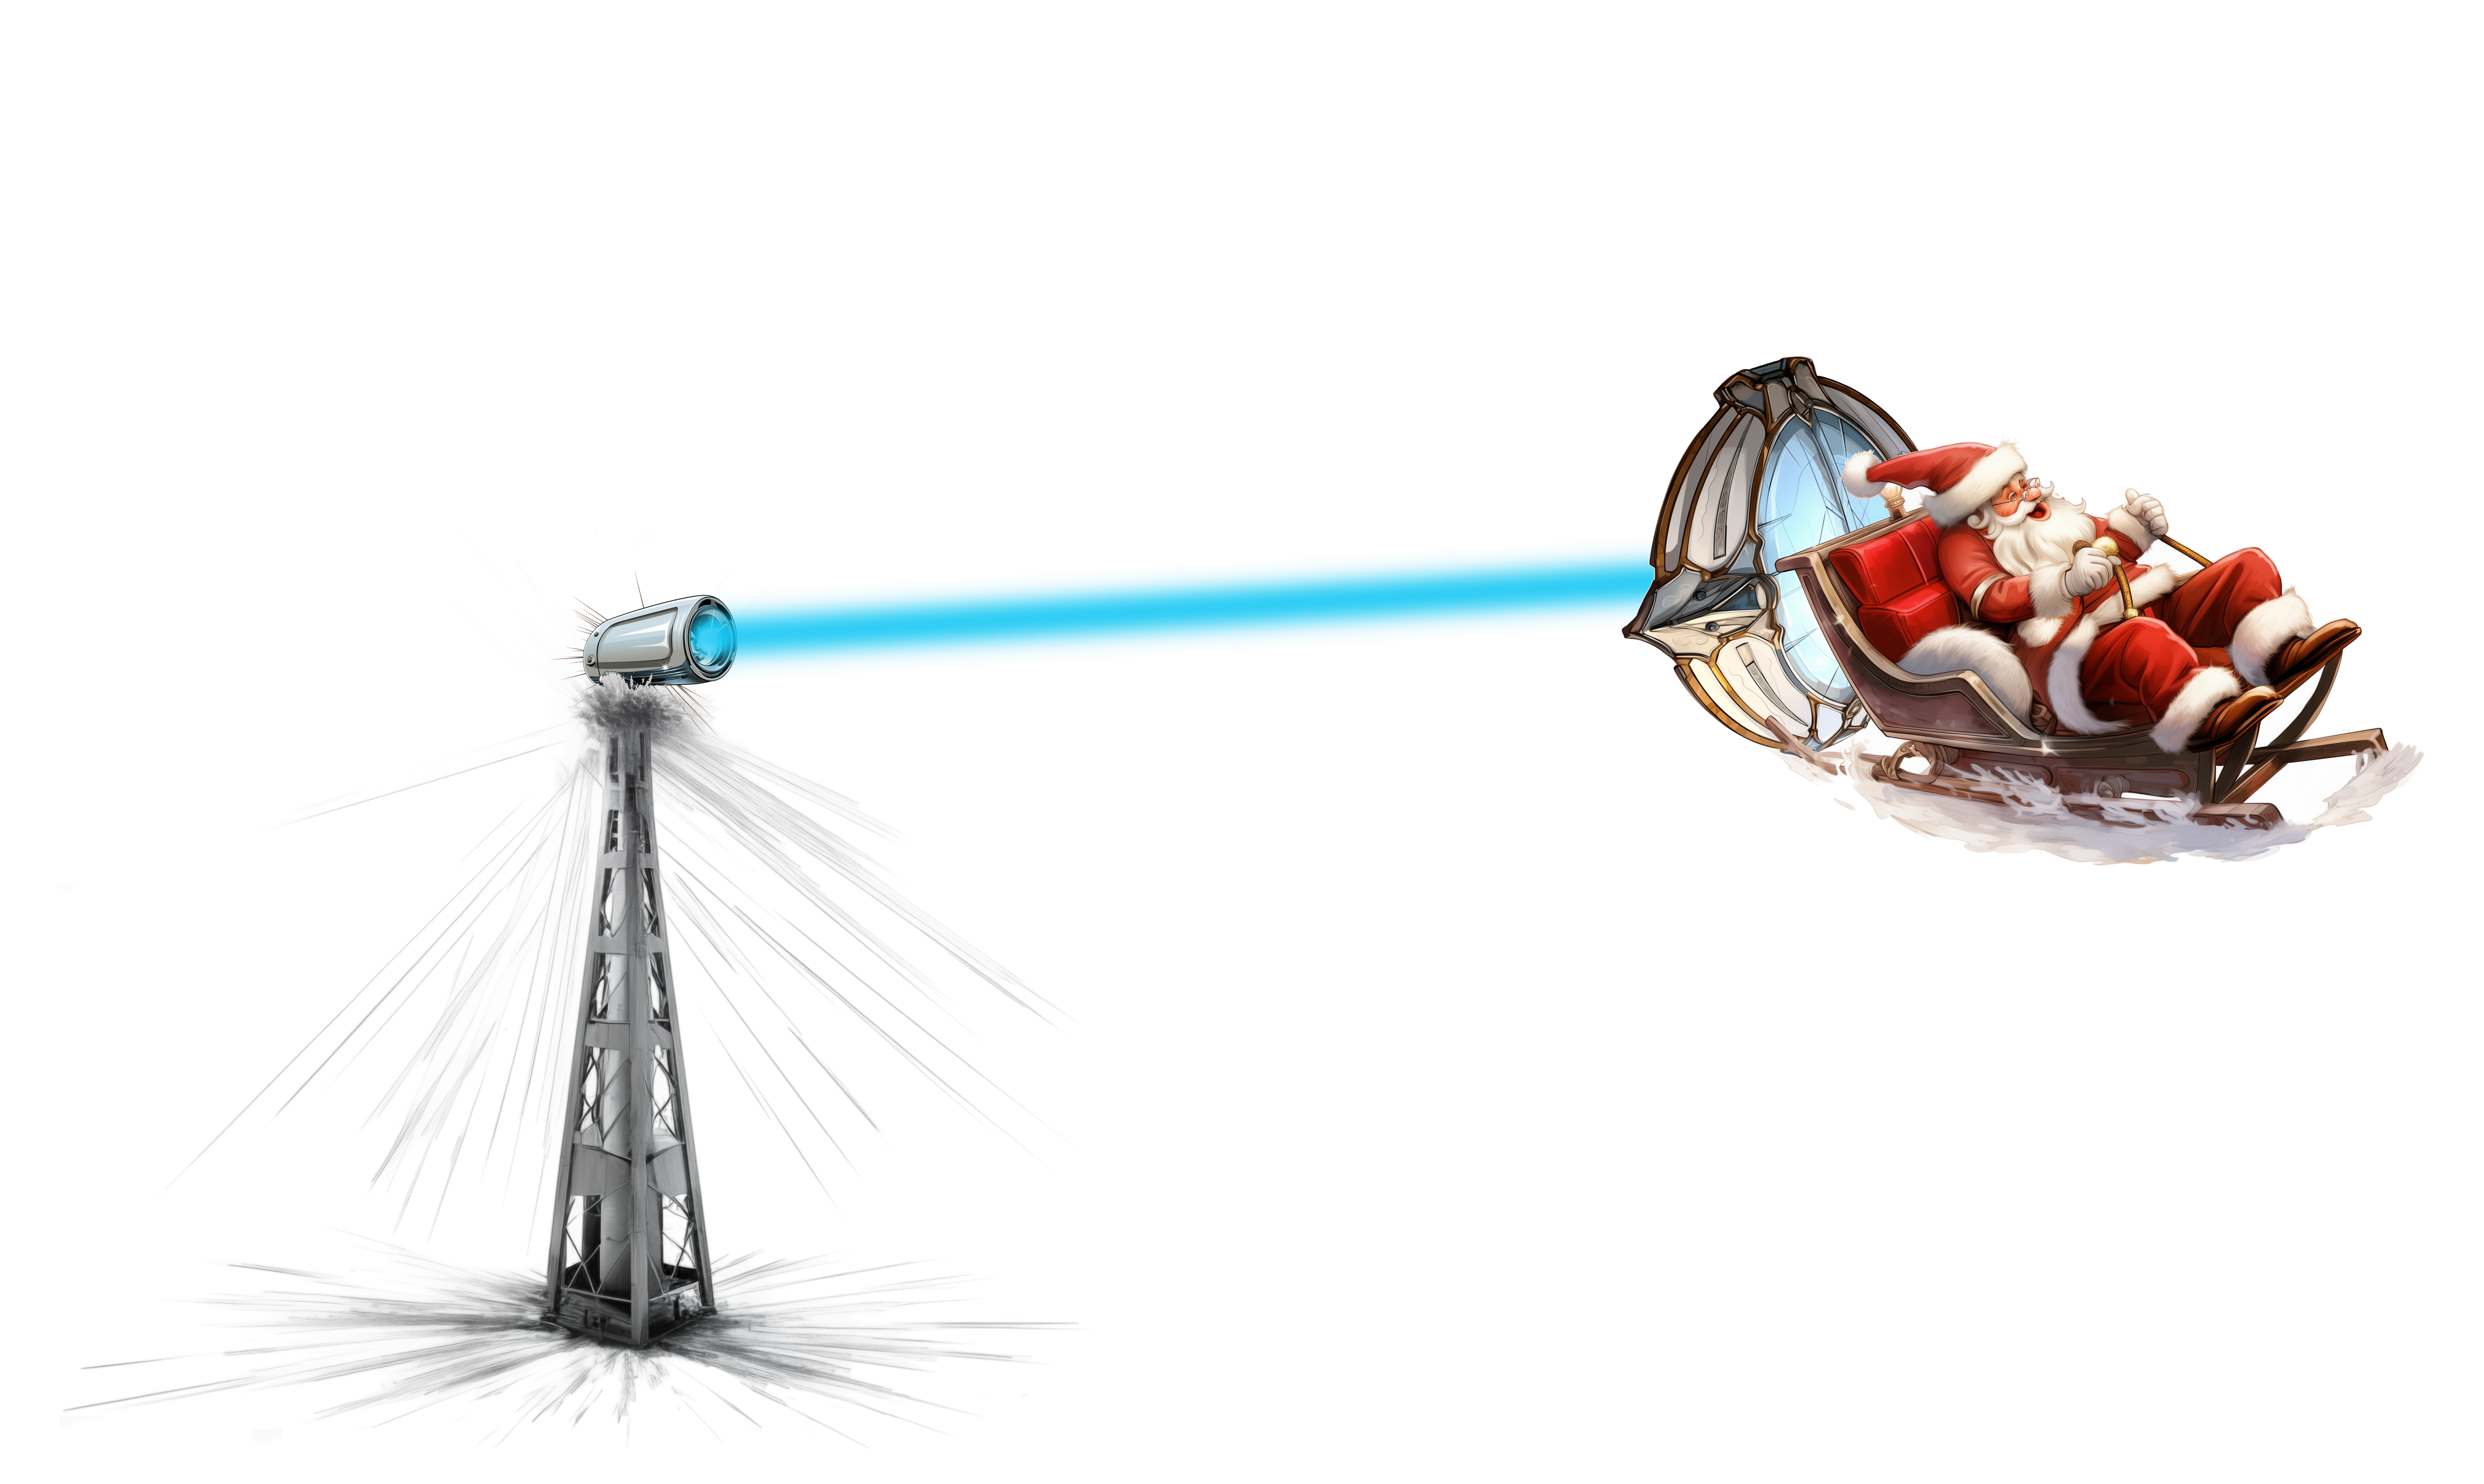
\includegraphics[width=\linewidth]{07full.png}\\
		Santa Clause trying his new high-tech sleigh.
	\end{center}
	
	If $D$ id the distance between the sleigh and the tower, the energy transmitted by the tower is proportional to $1/D$ (due to interaction of the laser with the atmosphere).
	The speed of the sleigh is proportional to the energy it receives from the tower.
	
	
\end{document}